% Author: Alfredo Sánchez Alberca (asalber@ceu.es)
% !TEX program = xelatex
\documentclass[a4paper, 10pt]{article}
\usepackage[top=2.5cm, bottom=3cm, left=2cm, right=2cm, headsep=1.5cm]{geometry}
\usepackage{amsmath}
%\usepackage{mathspec}
\usepackage[sfdefault,semibold,light]{FiraSans}
\usepackage{newtxsf}
\usepackage{multicol}
\usepackage{tikz}
\usepackage{graphicx}
\usepackage[most]{tcolorbox}
\usepackage[pdfauthor={Alfredo Sánchez Alberca}, pdftitle={Statistical formulas}, colorlinks=true]{hyperref}

% HEADER AND FOOT
\usepackage{fancyhdr}
\pagestyle{fancy}
\lhead{
\includegraphics{img/logo-uspceu.pdf}} 
\rhead{\url{http://aprendeconalf.es}}
\renewcommand{\headrulewidth}{0pt}
\renewcommand{\floatpagefraction}{.8}
\renewcommand{\textfraction}{.1}

% COLORS
\usepackage{xcolor}
\definecolor{color1}{RGB}{5,161,230} % Blue
\definecolor{color2}{RGB}{238,50,36} % Red
\definecolor{color3}{RGB}{0,205,0} % Green
\definecolor{color4}{RGB}{243,102,25} % Orange

% LISTS
\usepackage[shortlabels]{enumitem} % Customize lists
%\setlist{nolistsep} % Reduce spacing between bullet points and numbered lists
\setlist[description]{style=sameline,leftmargin=0cm}

% SECTIONS
\usepackage{titlesec}
\titleformat{\section}
{\color{color1}\normalfont\Huge\bfseries}
{\color{color1}\thesection}{1em}{}
\titleformat{\subsection}
{\color{color1}\normalfont\Large\bfseries}
{\color{color1}\thesubsection}{1em}{}

\setlength{\columnsep}{1cm}

\begin{document}
% !TEX root = statistics-formulas-cheatsheet.tex
% Author: Alfredo Sánchez Alberca (asalber@ceu.es)

\sloppy

\section*{Statistics Formulas}

\footnotesize
\tcbset{enhanced, colback=color1!10, colframe=color1, fonttitle=\bfseries\large\sffamily}

\begin{multicols*}{2}

\subsection*{Descriptive Statistics}

\begin{tcolorbox}[hbox, title=Frequencies]
\begin{minipage}{0.4\textwidth}
\begin{description}
\item [Sample size] $n$ num of individuals in the sample.
\end{description}
\begin{description}
\item [Absolute frequency] $n_i$ (num of $x_i$ in the sample)
\item [Relative frequency] $f_i=n_i/n$
\item [Cumulative absolute freq] $N_i=\sum_{k=0}^in_i$
\item [Cumulative relative freq] $F_i=N_i/n$
\end{description}
\end{minipage}
\end{tcolorbox}

\begin{tcolorbox}[hbox, title=Central tendency statistics]
\begin{minipage}{0.4\textwidth}
\begin{description}
\item [Mean] $\bar{x}=\dfrac{\sum x_i}{n}$
\item [Median] $me$ The value with cum.rel.freq. $F_{me}=0.5$.
\item [Mode] $mo$ The most frequent value.
\end{description}
\end{minipage}
\end{tcolorbox}

\begin{tcolorbox}[hbox, title=Position statistics]
\begin{minipage}{0.4\textwidth}
\begin{description}
\item [Quartiles] $Q_1,Q_2,Q_3$ divide the distribution into 4 equal parts.
      Their cum.rel.freqs. are
      $F_{Q_1}=0.25$, $F_{Q_2}=0.5$ and $F_{Q_3}=0.75$.
\item [Percentiles] $P_1,P_2,\cdots,P_{99}$ divide the distribution into 100 equal parts.\\
      The cum.rel.freq. is $F_{P_i}=i/100$.
\end{description}

\textbf{Interpolation}

\resizebox{\textwidth}{!}{% Author: Alfredo Sánchez Alberca (asalber@ceu.es)

\pgfplotsset{
    standard/.style={
        axis x line=middle,
        axis y line=middle,
        % enlarge x limits=0.15,
        % enlarge y limits=0.15,
        every axis x label/.style={at={(current axis.right of origin)},anchor=north west},
        every axis y label/.style={at={(current axis.above origin)},anchor=north east}
    }
}

\begin{tikzpicture}
\begin{axis}[standard, xlabel={$X$}, ylabel={$F$}, axis equal, xmin=-0.1, xmax=7, ymin=0,
ymax=5, xtick={1,6}, xticklabels={$l_{i-1}$,$l_i$}, ytick={1,4}, yticklabels={$F_{i-1}$,$F_i$}]

\coordinate (A) at (axis cs:6,1);
\coordinate (B) at (axis cs:1,1);
\coordinate (C) at (axis cs:6,4);
\coordinate (D) at (axis cs:4,1);
\coordinate (E) at (axis cs:4,2.8);
\coordinate (F) at (axis cs:-0.1,2.8);
\coordinate (G) at (axis cs:4,-0.1);
\end{axis}

\draw (B) -- (C);

\draw[fill=color1!20] (A) -- (B) -- (C) -- cycle;
\draw[fill=color2!20] (D) -- (B) -- (E) -- cycle;

\tkzMarkAngle[fill= green!50,size=1cm](A,B,C)
\tkzLabelAngle[pos = 0.7](A,B,C){$\alpha$}
%\node[anchor=west] at (7,3) {$\color{color1} \displaystyle \tan(\alpha) = \frac{F_i-F_{i-1}}{l_i-l_{i-1}}$};

\node[anchor=east] at (F) {$\frac{i}{100}$};
\draw[dashed] (F) -- (E) -- (G);
\node[anchor=north] at (G) {\color{color2}$P_i$};

%\node[anchor=west] at (7,2) {$\color{color2} \displaystyle \tan(\alpha) = \frac{0.5-F_{i-1}}{Me-l_{i-1}}$};


\end{tikzpicture}}

\[P_i=l_i+\frac{\frac{i}{100}-F_{i-1}}{F_i-F_{i-1}}(l_i-l_{i-1})\]

\end{minipage}
\end{tcolorbox}

\begin{tcolorbox}[hbox, title=Dispersion statistics]
\begin{minipage}{0.4\textwidth}
\begin{description}
\item [Interquartile range] $IQR=Q_3-Q_1$
\item [Variance] $s^2=\dfrac{\sum (x_i-\bar x)^2}{n}=\dfrac{\sum x_i^2}{n}-\bar x^2$
\item [Standard deviation] $s=+\sqrt{s^2}$
\item [Coefficient of variation] $cv=\dfrac{s}{|\bar{x}|}$
\end{description}
\end{minipage}
\end{tcolorbox}

\begin{tcolorbox}[hbox, title=Shape statistics]
\begin{minipage}{0.4\textwidth}
\begin{description}
\item [Coefficient of skewness] $g_1=\dfrac{\sum(x_i-\bar{x})^3}{ns^3}$
\item [Coefficient of kurtosis] $g_2=\dfrac{\sum(x_i-\bar{x})^4}{ns^4}-3$
\end{description}
\end{minipage}
\end{tcolorbox}

\begin{tcolorbox}[hbox, title=Linear transformations]
\begin{minipage}{0.4\textwidth}
\begin{description}
\item[Linear transformation] $y=a+bx$
      \begin{align*}
      \bar y & = a+b\bar x \\
      s_y    & = bs_x
      \end{align*}
\item[Standarization] $z=\dfrac{x-\bar x}{s_x}$
\end{description}
\end{minipage}
\end{tcolorbox}


\subsection*{Regression and correlation}

\begin{tcolorbox}[hbox, title=Linear regression]
\begin{minipage}{0.4\textwidth}
\begin{description}
\item [Covariance] $s_{xy}=\dfrac{\sum x_iy_j}{n}-\bar{x}\bar{y}$
\item [Regression lines]:
      \begin{align*}
      \mbox{$y$ on $x$} & : y=\bar{y}+\dfrac{s_{xy}}{s_x^2}(x-\bar{x}) \\
      \mbox{$x$ on $y$} & : x=\bar{x}+\dfrac{s_{xy}}{s_y^2}(y-\bar{y})
      \end{align*}
\item [Regression coefficients]
      \[
      \mbox{($y$ on $x$) } b_{yx}=\dfrac{s_{xy}}{s_x^2}\quad \mbox{($x$ on
      $y$) } b_{xy}=\dfrac{s_{xy}}{s_y^2}
      \]
\item[Coefficient of determination]
      \[r^2=\dfrac{s_{xy}^2}{s_x^2s_y^2} \qquad 0\leq r^2\leq 1\]
\item[Correlation coefficient]
      \[r=\dfrac{s_{xy}}{s_xs_y}.\qquad -1\leq r\leq 1\]
\end{description}
\end{minipage}
\end{tcolorbox}

\medskip

\begin{tcolorbox}[hbox, title=Non-linear regression]
\begin{minipage}{0.4\textwidth}
\begin{description}
\item[Exponential model] $y=e^{a+bx}$\\
      Apply the logarithm to the dependent variable and compute the line $\log y = a+bx$.
\item[Logarithmic model] $y=a+b\log x$\\
      Apply the logarithm to the independent variable and compute the line $y=a+b\log x$.
\item[Potential model] $y=ax^b$\\
      Apply the logarithm to both variables and compute the line $\log y = a+b\log x$.
\end{description}
\end{minipage}
\end{tcolorbox}

\newpage

\subsection*{Probability}

\begin{tcolorbox}[hbox, title=Event operations]
\begin{minipage}{0.4\textwidth}
\textbf{Union}
\begin{center}
% Author: Alfredo Sánchez Alberca (asalber@ceu.es)
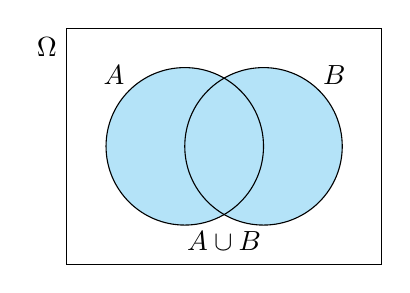
\begin{tikzpicture}
\def\firstcircle{(1.5,1.5) circle (1cm)}
\def\secondcircle{(2.5,1.5) circle (1cm)}

\fill[color1!30] \firstcircle;
\fill[color1!30] \secondcircle;
\draw (0,3) node[anchor=north east] {$\Omega$} rectangle (4,0);
\draw \firstcircle node[xshift=-0.9cm, yshift=0.9cm] {$A$};
\draw \secondcircle node[xshift=0.9cm, yshift=0.9cm] {$B$};

\node at (2,0.3) {$A\cup B$};
\end{tikzpicture}
\end{center}
\textbf{Intersection}
\begin{center}
% Author: Alfredo Sánchez Alberca (asalber@ceu.es)

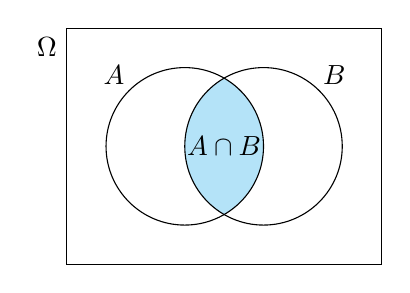
\begin{tikzpicture}
\def\firstcircle{(1.5,1.5) circle (1cm)}
\def\secondcircle{(2.5,1.5) circle (1cm)}

\begin{scope}
\clip \firstcircle;
\fill[color1!30] \secondcircle;
\end{scope}

\draw (0,3) node[anchor=north east] {$\Omega$} rectangle (4,0);
\draw \firstcircle node[xshift=-0.9cm, yshift=0.9cm] {$A$};
\draw \secondcircle node[xshift=0.9cm, yshift=0.9cm] {$B$};

\node at (2,1.5) {$A\cap B$};
\end{tikzpicture}
\end{center}
\textbf{Complement}
\begin{center}
% Author: Alfredo Sánchez Alberca (asalber@ceu.es)

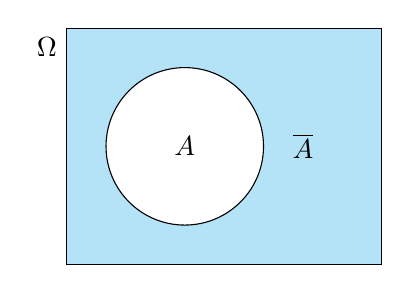
\begin{tikzpicture}
\def\circle{(1.5,1.5) circle (1cm)}
\def\rectangle{(4,0) rectangle (0,3)}

\begin{scope}[even odd rule]
\clip \circle (0,0) rectangle (4,3);
\fill[color1!30] \rectangle;
\end{scope}

\draw \rectangle node[anchor=north east] {$\Omega$};
\draw \circle node {$A$};
\node at (3,1.5) {$\overline A$};
\end{tikzpicture}
\end{center}
\textbf{Difference}
\begin{center}
% Author: Alfredo Sánchez Alberca (asalber@ceu.es)

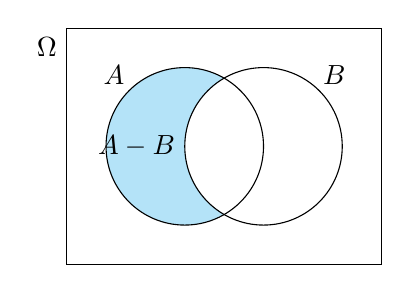
\begin{tikzpicture}
\def\firstcircle{(1.5,1.5) circle (1cm)}
\def\secondcircle{(2.5,1.5) circle (1cm)}

\begin{scope}[even odd rule]
\clip \secondcircle (0,0) rectangle (4,3);
\fill[color1!30] \firstcircle;
\end{scope}

\draw (0,3) node[anchor=north east] {$\Omega$} rectangle (4,0);
\draw \firstcircle node[xshift=-0.9cm, yshift=0.9cm] {$A$};
\draw \secondcircle node[xshift=0.9cm, yshift=0.9cm] {$B$};

\node[anchor=east] at (1.5,1.5) {$A-B$};
\end{tikzpicture}
\end{center}
\end{minipage}
\end{tcolorbox}

\begin{tcolorbox}[hbox, title=Algebra of events]
\begin{minipage}{0.4\textwidth}
\begin{description}
\item[Idempotency] $A\cup A=A$,\quad $A\cap A=A$
\item[Commutative] $A\cup B=B\cup A$,\quad $A\cap B = B\cap A$
\item[Associative] $(A\cup B)\cup C = A\cup (B\cup C)$,\quad $(A\cap B)\cap C = A\cap (B\cap C)$
\item[Distributive] $(A\cup B)\cap C = (A\cap C)\cup (B\cap C)$,\quad $(A\cap B)\cup C = (A\cup C)\cap (B\cup C)$
\item[Neutral element] $A\cup \emptyset=A$,\quad $A\cap \Omega=A$
\item[Absorbing element] $A\cup \Omega=\Omega$,\quad $A\cap \emptyset=\emptyset$.
\item[Complementary symmetric element] $A\cup \overline A = \Omega$,\quad $A\cap \overline A= \emptyset$
\item[Double contrary] $\overline{\overline A} = A$
\item[Morgan's laws] $\overline{A\cup B} = \overline A\cap \overline B$,\quad $\overline{A\cap B} = \overline A\cup \overline B$
\end{description}
\end{minipage}
\end{tcolorbox}

\begin{tcolorbox}[hbox, title=Basic probability]
\begin{minipage}{0.4\textwidth}
\begin{description}
\item [Union] $P(A\cup B)=P(A)+P(B)-P(A\cap B)$
\item [Intersection] $P(A\cap B)=P(A)P(B|A)$
\item [Difference] $P(A-B)=P(A)-P(A\cap B)$
\item [Contrary] $P(\overline{A})=1-P(A)$
\end{description}
\end{minipage}
\end{tcolorbox}

\begin{tcolorbox}[hbox, title=Conditional probability]
\begin{minipage}{0.4\textwidth}
\begin{description}
\item [Conditional probability] $P(A|B)=\dfrac{P(A\cap B)}{P(B)}$
\item [Independent events] $P(A|B)=P(A)$.
\item [Total probability Theorem] \[P(B)=\sum_{i=1}^n P(A_i)P(B|A_i)\]
\item [Bayes Theorem] \[P(A_i|B)=\dfrac{P(A_i)P(B|A_i)}{\sum_{i=1}^n P(A_i)P(B|A_i)}\]
\end{description}
\end{minipage}
\end{tcolorbox}


\begin{tcolorbox}[hbox, title=Risks]
\begin{minipage}{0.4\textwidth}
\begin{center}
\begin{tabular}{|l|c|c|}
\cline{2-3}
\multicolumn{1}{c|}{} & $E$ & $\overline E$ \\
\hline
Treatment             & $a$ & $b$           \\
\hline
Control               & $c$ & $d$           \\
\hline
\end{tabular}
\end{center}
\begin{description}
\item[Prevalence] Proportion of individuals with $E$: $P(E)$
\item[Incidence rate or absolute risk] $R(E)=\dfrac{a}{a+b}$
\item[Odds] $O(E)=\dfrac{a}{b}$
\item[Relative risk] $RR(E)=\dfrac{a/(a+b)}{c/(c+d)}$
\item[Odds ratio] $OR(E)=\dfrac{a/b}{c/d}=\dfrac{a\cdot d}{b\cdot c}$
\end{description}
\end{minipage}
\end{tcolorbox}


\begin{tcolorbox}[hbox, title=Diagnostic tests]
\begin{minipage}{0.4\textwidth}
\begin{center}
\begin{tabular}{|l|c|c|}
\cline{2-3}
\multicolumn{1}{c|}{} & Disease $D$ & No disease $\overline D$ \\
\hline
Test $+$              & $VP$        & $FP$                     \\
\hline
Test $-$              & $FN$        & $VN$                     \\
\hline
\end{tabular}
\end{center}
\begin{description}
\item[Sensitivity] $P(+|D)=\dfrac{VP}{VP+FN}$
\item[Specificity] $P(-|\overline{D})=\dfrac{VN}{FP+VN}$
\item[Positive Predictive Value (PPV)] $P(D|+)=\dfrac{VP}{VP+FP}$
\item[Negative Predictive Value (NPV)] $P(\overline{D}|-)=\dfrac{VN}{FN+VN}$
\item[Positive Likelihood Ratio (LR+)] $\dfrac{P(+|D)}{P(+|\overline{D})}$
\item[Negative Likelihood Ratio (LR-)] $\dfrac{P(-|D)}{P(-|\overline{D})}$
\end{description}
\end{minipage}
\end{tcolorbox}


\subsection*{Random Variables}

\begin{tcolorbox}[hbox, title=Discrete]
\begin{minipage}{0.4\textwidth}
\begin{description}
\item [Binomial probability function $B(n,p)$]
      \[f(x)=\binom{n}{x}p^x (1-p)^{n-x}=\dfrac{n!}{x!(n-x)!}p^x (1-p)^{n-x}\]
\item [Poisson probability function $P(\lambda)$]
      \[f(x)=e^{-\lambda}\frac{\lambda^x}{x!}\]
\item [Law of rare events] $B(n,p)\approx P(np)$ for $n\geq 30$ and $p\leq 0.1$.
\end{description}
\end{minipage}
\end{tcolorbox}

\begin{tcolorbox}[hbox, title=Continuous]
\begin{minipage}{0.4\textwidth}
\begin{description}
\item[Normal $N(\mu,\sigma)$]
      \[f(x)= \frac{1}{\sigma\sqrt{2\pi}}e^{-\frac{(x-\mu)^2}{2\sigma^2}}\]
      \textbf{Standard normal $N(0,1)$}
\item[Chi-square $\chi^2(n)$]
      \[X = Z_1^2+\cdots +Z_n^2,\]
      where $Z_i\sim N(0,1)$.
\item[Student's t $T(n)$]
      \[T = \frac{Z}{\sqrt{X/n}},\]
      where $Z\sim N(0,1)$ and $X\sim \chi^2(n)$.
\item[Fisher's F $F(n,m)$]
      \[F = \frac{X/m}{Y/n},\]
      where $X\sim \chi^2(m)$ and $Y\sim \chi^2(n)$.
\end{description}
\end{minipage}
\end{tcolorbox}

\end{multicols*}
\end{document}

